\input{chapter-header.tex}
% ===========================================================================
\chapter{Achieving Software Evolution with Object Spaces}
\minitoc
% ===========================================================================
\introduction
% ===========================================================================

We will present three techniques for software evolution, and how their challenges are overcame with our object spaces model: bootstrapping, tailoring, runtime monitoring and modification.

% ===========================================================================
\section{Bootstrapping}
% ===========================================================================

The concept of \emph{bootstrap} is  well known in the context of compilers. For example, a bootstrapped C compiler is a compiler that, by using its own source code, can produce another compiler with its same behavior. We can generalize the process to obtain a bootstrapped system as the following.

\begin{definition}[Bootstrap Process]
A bootstrap is a process that defines a system S using S itself, by providing a self-describing specification of its own structure and behavior.
Alternatively, we can say a bootstrap is a process that defines a system S using a specification that can be fully processed by S itself.
\end{definition}

Once bootstrapped, a system relies only on itself and its specification to re-generate its own infrastructure.
Improvements such as bugfixing, speed optimizations and mutations of the language are performed by modifying the specification and recreating the system. 
We can thus define a bootstrapped system as the following. 

\begin{definition}[Bootstrapped System]
A bootstrapped system is a system that supports its own evolution.
\end{definition}

\subsection{Evolution by Bootstrapping}

When the system in construction is introduced into its own recreation process, this process is named a \emph{bootstrap}. The most prominent example is the C compiler which was initially developed in another language, and later rewritten in the C language itself and used to compile itself.  In an informal way, a bootstrap is the process to use the system being developed as early as possible to define this exact system. The key idea is to be able to use the new abstractions provided by the new system as early as possible and also to support the modification of the system. This way, the system can benefit from its expressive power and abstractions to evolve.

Bootstrapping a system provides a deterministic, explicit and self-describing process for generating an autonomous reflective object-oriented system. Its direct benefit is the generation of a complete self-description of the system, which can be manipulated by the system itself.
The self-description eases the understanding of the system by using the abstractions it provides to define itself. A key advantage is the description of its meta-circularities, the initialization of the system and how they are solved.

Besides understanding, bootstrapping supports the evolution of a system. Once bootstrapped, the specification of the system can be easily modified to make possible deep changes to the system.
For example, a system may change its object model or layout of objects in memory.

Bootstrapping a system may be perceived as an academic exercise but it has strong software engineering positive properties: 

\begin{description}
\item[Enforces a self description.] A bootstrapped system can describe and manipulate itself. This means that the abstractions existent in the system can be used in the definition of the system, providing a more powerful way to describe the system.

 \item[Provides an agile and explicit process.] Having a bootstrap is important to be sure that the system can always be built from the ground.  
It makes sure that initialization of key parts of the system is exercised each time the system is built. It limits broken and outdated code of the system initialization. It also makes sure that there is no hidden dependency. This also supports the idea of software construction by selecting and assembling elements. 
 
\item[Warranties initial state.] A system built from the ground by using the same specification and builder should have a deterministic behavior and initial state.  

\item[Supports explicit malleability and evolution.] Having an explicit and operational machine executable process to build a kernel is also important to support a system's evolution \cite{Casa09a}. The evolution can be achieved by defining new entities and their relationships with existing ones inside the specification describing the system. There is no need to build transition paths from an existing system to the next version. This is particularly important for radical changes where the migration would be too complex.
 
\end{description}

\subsection{A Bootstrapping Process for Reflective Languages}\label{sec:model}

A reflective object-oriented system is a reflective system where its entities are represented by objects. This objects are causally connected so they are able of reasoning about and acting upon themselves.
The causal connections create a peculiar relation between reflective systems and their specification: a reflective object-oriented system contains a \emph{reified} version of its own structure and behavior.
For example, they contain meta-objects representing entities such as classes, instance variables, packages or methods.
Meta-objects insert the idea of meta-circularity in the reflective system: a meta-object is an object, and it is also described by a meta-object.
Introspection and self-modification in reflective object-oriented systems are the result of respectively querying and mutating these meta-objects.

Though reflective object-oriented systems reflect their own structure and behavior, they do not mandatory reflect the process to build and initialize themselves.
A bootstrap for an object-oriented reflective system must ensure the meta-circularities of the system are closed and introduce this process in the system.
Thus, we can define the bootstrap of an object-oriented reflective system as the following.

\begin{definition}[Bootstrap Process for an Object-Oriented System]
A bootstrap of an object-oriented reflective system is a process that defines an object-oriented system S using S itself, by reifying the structure and behavior of the system in itself.
\end{definition}

\begin{definition}[Bootstrapped Object-Oriented Reflective System]
A bootstrapped object-oriented reflective system is a bootstrapped object-oriented system capable of reasoning about and acting upon itself in order to evolve.
\end{definition}

In particular, the specification describing an object-oriented reflective system must contain:
\begin{description}
\item \textbf{The Structure of the system.}
The entities and connections conforming the structure of the system and their behavior.
For example, classes, metaclasses and methods are described to define the entities of the system. Additionally, their relations such as superclass and subclass are described since they are needed to assemble the system.

\item \textbf{The initialization order of the system.}
The specification must express how to initialize the system.
Some initializations are coupled, so their order must be specified.
For example, an object A must be mandatory initialized before another object B, because B uses A.
\end{description}

\subsubsection{Overview}
Hazelnut is a \emph{system builder} that performs the bootstrap process of an object-oriented reflective system out of an existing reflective system: Pharo.
We will refer to Pharo as the \emph{source system} from where the \emph{new system} will be created.
Hazelnut takes advantage of the reflective capabilities of the source system to perform tasks such as create classes, compile methods and modify the system structure.

Hazelnut defines both a builder and a specification model that can be used to generate object-oriented reflective systems.
The specification describes both the structure and behavior of the bootstrapped system, as well as part of the process to build it.

The structure and behavior of the system is described as class and methods declarations in files. For example, \autoref{code:spec_extract} exemplifies the structural specification with an extract of the \ct{Point} declarations. The \ct{Point} class is described specifying its superclass, instance variables, and package. The source code of the class' methods are also included in this part of the specification.

\begin{figure}[!ht]
				\begin{code}
				 Class
				    name: #Point;
				    superclass: #Object;
				    instanceVariables: #(#x #y);
				    package: #'Kernel-BasicObjects'.

				 Class Point >> corner: aPoint
				   [
				   ^ Rectangle origin: self corner: aPoint
				   ]
				   
				 Class Point >> dist: aPoint
				   [
				    | dx dy |
				    dx := aPoint x - x.
				    dy := aPoint y - y.
				    ^ (dx squared + dy squared) sqrt
				   ]
				\end{code}

\caption{Extract of \ct{Point} class definition in the structural part of the bootstrap specification \label{code:spec_extract}}
\end{figure}

On the other hand, the initialization process of the system is described as a \emph{specification object}. The Hazelnut builder delegates the particular parts of the initialization process of the new system to this specification object. 
The resulting new system is a reflective object-oriented system, reifying its own structure and behavior in a causal connected way. It will contain all the objects needed to run independently of the source system. The resulting reflective system, again, does not mandatory describe the process to rebuild itself.
Hazelnut achieves the creation of the new system by creating a new namespace in the source system.
This new space represents the new system.
It co-exists side by side with the source system, on top of the same Virtual Machine.
Hazelnut takes the specification of the new system and builds all the corresponding objects:
each class and object defined in the specification will have an alive counterpart residing in the new system.

The key benefit of having two systems side by side is that objects of the new system are able to receive messages during the construction.
Encapsulation and polymorphism ease their manipulation.
Without this capability, objects should be manipulated as raw data structures without behavior. This supposes a problem when modifying complex objects such as a \ct{Dictionary} because all the code to maintain coherent its internal structure should be rewritten.

Regarding the meta-circularities, during the first stages of the construction of the new system, objects in the new system reference \emph{temporary} objects from the source system.
Temporary objects are polymorphic with objects in the new system, so the new objects can delegate to them perceiving no difference.
Thus, they allow objects in the new system to perform some tasks while still partially initialized.
When the new system is ready, references to temporary objects are replaced by references to objects in the new system.
The new system is independent of the source system and we consider it bootstrapped. For example, the ObjVLisp~\cite{Coin87a} bootstrap solves the meta-circularity problems by creating a first temporary version of the class \ct{Class} (not using inheritance) using low level API.
The class \ct{Object} is created as an instance of the first class \ct{Class}. Finally, \ct{Class} is reimplemented using the first one and this time inheriting from \ct{Object}.

\subsubsection{Bootstrap process of Hazelnut}
Hazelnut defines the following process to bootstrap a reflective system, as illustrated in \autoref{fig:hazelnut_overview}. Each of the steps will be fully explained while presenting the Pharo bootstrap in the next section. 

\begin{itemize}
\item \textbf{Step 1: Load specification.}
The specification describing the system is read by  Hazelnut. Each entity appearing in the specification is reified into Hazelnut as a \emph{specification object}. For example, a class described in the specification will be transformed into a class definition in hazelnut. 

\item \textbf{Step 2: Solve Basic Structural Meta-circularity.}
A reflective system meta-level is created by causally connected objects ending up in meta-circularities.
This step is responsible for solving the basic meta-circularity of the system, which is the minimal structural part of it enabling the construction of the rest of the system.
For example, in order to create a class for a Smalltalk system, the class \ct{Metaclass} and its class should exist. Thus, this step involves the creation of the first \ct{Metaclass}, which in the upcoming steps will be used to define new classes.
This first structural objects will refer to temporary objects of the source system after this step.

\item \textbf{Step 3: Build Class Shells.}
In this step the skeleton of all classes of the new system are created. These skeletons act as \emph{class shells} since they have the structure of a class, but do not yet contain all the information they need to work. 
The creation of class shells is delegated to the hazelnut class definitions loaded during the step 1 of the process.
The class shells created in this step are partially initialized with temporal objects from the source system and do not have methods installed in them yet.
Relations between the class shells --such as superclass/subclass-- are not set in this step, so it can be performed independently of any order.
Class shells will be filled in the following steps to become fully functional classes.

\item \textbf{Step 4: Install Methods.}
Once all class shells are built, methods are created and installed into their respective owners. Depending on the format of the specification, method building relies on compiling source code or loading pre-compiled binary code. In case of building a system with a different semantics or byte-codes, a cross-compiler inside the source system can be used to compile the methods source code.

\item \textbf{Step 5: Complete Initialization of the new System.}
In this step, the initialization of the new system is completed.
The class shells are filled, and the relation between them are set.
Other state of the system is initialized. For example, the objects representing the packages of the system could be created.
Initializations of this step are performed by the collaboration of the source and the new system, until the new system is completely independent and isolated from the source system.

\end{itemize}

\begin{figure}[!ht]
\begin{center}
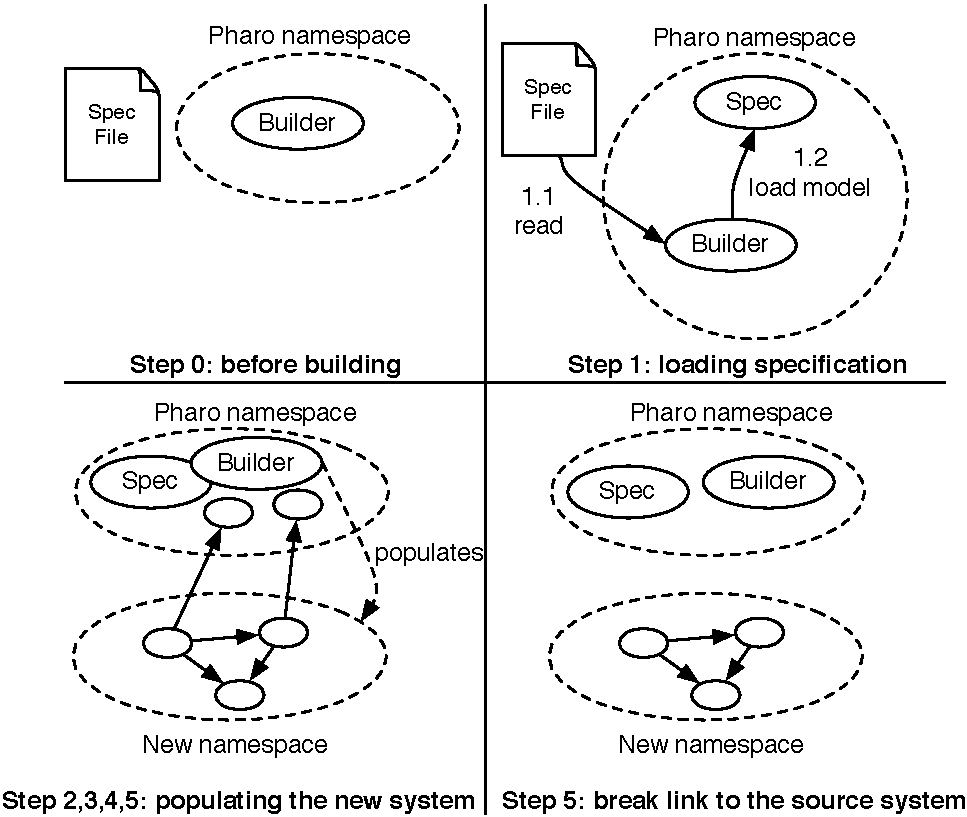
\includegraphics[width=0.6\linewidth]{hazelnut_overview}
\caption{Overview of Hazelnut process to bootstrap a reflective system\label{fig:hazelnut_overview}}
\end{center}
\end{figure}

% ===========================================================================
\subsection{Challenges of Bootstrapping a Reflective Object-Oriented System}
% ===========================================================================

Meta-circularities make the process of building a new reflective system more complex than building a system without them. 
The building process should solve these meta-circularities and provide a working system.
Once solved, we say the meta-circularities are \emph{closed}.
Meta-circularities in a reflective system such can be illustrated with several examples:

\begin{description}
\item \emph{Reflective core are expressed in themselves.} The core of many reflective and dynamic languages such as 
Ruby, Smalltalk and even Java are self-referencing. For example, the \ct{Metaclass} class is an instance of the \ct{Metaclass} metaclass and vice versa, as shown in \autoref{fig:smalltalk_metacircularity}.
This leads to a recursive dilemma: how can each of these two entities be initially built without its defining pair.
Due to its importance in the system structure this meta-circularity should be mandatory solved during the first steps of the bootstrap. We call this, the \emph{basic structural meta-circularity} of the system.

\item \emph{Finding the order of construction is complex.} A class must receive the \ct{new} message to create a new object.
A method with the same selector is looked up in the class' metaclass hierarchy.
Since methods are objects, they have to be instantiated also.
The meta-circularity resides in the fact a first \ct{new} method should exist to define all methods.
\end{description}

Such self-references are also present in other languages with reflective capabilities: \eg in Java the ClassLoader is a class itself;
Ruby presents an object-model very similar to Smalltalk extended with mixins.

\begin{figure}[!ht]
\begin{center}
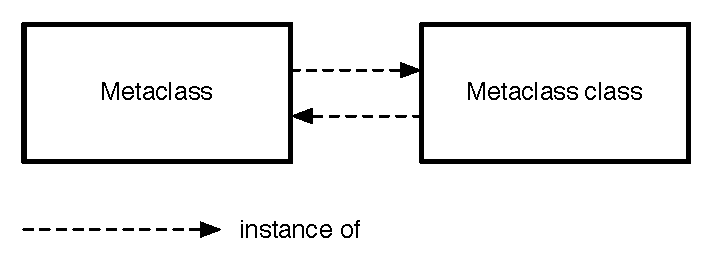
\includegraphics[width=0.40\linewidth]{smalltalk_metacircularity}
\caption{Smalltalk Metaclass circularity.\label{fig:smalltalk_metacircularity}}
\end{center}
\end{figure}

% ===========================================================================
\subsection{Object Spaces for Bootstrapping}
% ===========================================================================

lalala

% ===========================================================================
\section{Tailoring}
% ===========================================================================


% ===========================================================================
\subsection{Evolution by Tailoring} \label{sec:example_intro}
% ===========================================================================

% ===========================================================================
\subsection{Reducing an Application's Memory Footprint, a Motivating Example} \label{sec:example_intro}
% ===========================================================================

To clearly show the problem, consider the application using a logging library in Figure~\ref{fig:example_dead_code}.
An interface is present in the diagram to show polymorphism between two classes that do not share a class inheritance hierarchy. 
However, some languages, such as the dynamically typed ones, may not need to represent it in the source code.

\begin{figure}[ht]
\begin{center}
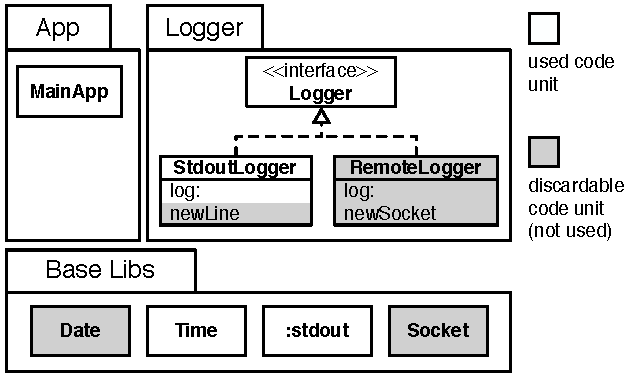
\includegraphics[width=.9\linewidth]{example_dead_code}
\caption{\small\textbf{Example of unused code units.} In gray, the unused code units that can safely be removed.\label{fig:example_dead_code}}
\end{center}
\end{figure}

Figure~\ref{fig:code_example1} shows the code of this application, written in the Pharo Smalltalk language. This application contains a \ct{MainApp} class with a \ct{start} method, which is the entry point of our application. The \ct{start} method creates an instance of \ct{Stdout\-Logger} and logs the application's start and end. In turn, the \ct{StdoutLogger} uses the \ct{stdout} global instance to log in the standard output the current time and the message. To print the time, the \ct{StdoutLogger} makes use of the \ct{Time} class from the base libraries of the language. Note that for the sake of clarity, we didn't include in the example all base libraries, though, in modern programming languages they represent a large codebase with several features going from networking to multithreading. For example, Java 8 SE contains 4240 classes\footnote{according to the javadoc API}, and the development edition of Pharo 2.0 contains 3342 classes and traits.

\begin{figure}[ht]
\begin{code}
MainApp>>start
    logger := StdoutLogger new.
    logger log: 'Application has started'.
    "do something"
    logger log: 'Application has finished'.

!\unusedcode{StdoutLogger>>newLine}!
!\unusedcode{~~~stdout newLine.}!

StdoutLogger>>log: aMessage
    stdout nextPutAll: Time now printString.
    stdout nextPutAll: aMessage.
    stdout newLine.
    
!\unusedcode{RemoteLogger>>log: aMessage}!
!\unusedcode{~~~| socket |}!
!\unusedcode{~~~socket := self newSocket.}!
!\unusedcode{~~~socket nextPutAll: Time now printString.}!
!\unusedcode{~~~socket nextPutAll: aMessage.}!
!\unusedcode{~~~socket newLine.}!

!\unusedcode{RemoteLogger>>newSocket}!
!\unusedcode{~~~"...."}!
!\unusedcode{~~~"creates an instance of socket given some configuration"}!
\end{code}

\caption{ \small\textbf{Code of the unused code units example.} In gray, methods not used by the application.\label{fig:code_example1}}
\end{figure}

In this example we can detect the following unused code units, shown in grey in Figure~\ref{fig:example_dead_code} and Figure~\ref{fig:code_example1}:
\begin{enumerate}
\item The logger library includes two logging classes~(\ct{Stdout\-Logger} and \ct{RemoteLogger}). Only the \ct{StdoutLogger} is used and thus, the \ct{RemoteLogger} class can be discarded.
\item Since the \ct{MainApp} class does not use the \ct{Socket} class nor the \ct{RemoteLogger} class~(the only user of the \ct{Socket} class), the \ct{Socket} class can be discarded.
\item No class in the application makes use of the \ct{Date} class. Then, this class can be safely removed.
\item The method \ct{newLine}~(lines 7-8 of Figure~\ref{fig:code_example1}) of the \ct{StdoutLogger} class is not used and can be also removed.
\item The \ct{StdoutLogger} class uses the \ct{Time} class to print the current time. Then, all code units that are not related to the \ct{Time now} resolution or printing~(\ie time arithmetic) could be considered as unused.
\end{enumerate}

We would like to generate a new version of this application not containing these unused code units while keeping the application's behavior. We call this technique \emph{Deployment Unit Tailoring} or \emph{Application Tailoring}.

% ===========================================================================
\subsection{A Tailoring Process for Reflective Languages}
% ===========================================================================

This paper describes \emph{Tornado}: an alternative solution to dead code elimination using a dynamic technique.
Tornado uses a run-fail-grow technique to identify during runtime those code units that are actually used in an application.
It consists in ``growing'' a seed into a deployable specialized version of an application. 
We feed this \emph{new} minimal version of the application (the \emph{seed}) with the missing code units needed to run.
The resulting deployable application only embeds the seed and used code.
By carefully choosing the seed, the user customizes the scope of the tailoring process making possible different levels of tailoring.
For example, a seed that includes all base libraries makes the tailoring process to only select used code in the application-specific part; whereas an empty seed makes the tailoring process to select used code in all parts: base libraries, application libraries and application-specific part.
% For example, if the seed includes the language base libraries, it ensures that the deployed application will have it all whereas an empty seed will result that only part of the base libs 
% Afterwards, deployment units are created from this shrank application to only contain the used code units.
% Using these compacted deployment units leverages the targeted device limitations. 
The dynamic nature of our solution allows its usage in dynamic languages, without type annotations. Our solution does not need to modify the original application thanks to its run-fail-grow approach.
It also successfully deals with applications that make use of programming language features such as reflection or open classes.


We propose Tornado, a run-fail-grow approach for tailoring. Tornado works by launching a \emph{nurtured} application that has only part of its required code units installed and a \emph{reference} application encompassing all the code units that resulted from the development process. When a failure is detected in the nurtured application, Tornado takes the missing code units from the reference application and install them into the nurtured application. Thus, the nurtured application grows progressively as failures are found.
Once finished, the nurtured application is ready to be deployed on target devices. Figure~\ref{fig:runfail} depicts the basics of our run-fail-grow approach.

%, in contrast with a trace-copy approach. Our run-fail approach avoids changing or manipulating the reference application, remaining unchanged from its original version.

\begin{figure}[ht]
\begin{center}
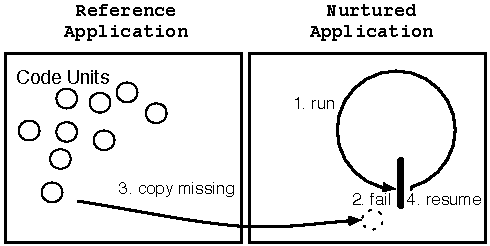
\includegraphics[width=.9\linewidth]{runfail}
\caption{\small \textbf{Application tailoring with a run-fail-grow approach.} We run the nurtured application~(1) and detects the missing units on failure~(2). At each failure, missing code units are installed from the reference application~(3) and the execution is resumed (just before the failure)~(4) until the process finishes. \label{fig:runfail}}
\end{center}
\end{figure}

% containing only \emph{application's entry points} (code units used to launch the application) 

Tornado starts by launching the reference application to create initial objects and perform startup computations. The reference application is then paused so its state do not change during the tailoring process. Pausing consists in suspending all processes and threads from the application.

Initially, the nurtured application is initialized with only a \emph{seed} embedding code units that developers want to ensure into the deployed application.
When the nurtured application starts from a seed that contains the language base libraries, the tailoring will only affect the application specific code units and third-party libraries.
When it starts from an empty seed, it will also tailor base libraries.

Following, it installs one or more \emph{application's entry points}.
An application's entry point consists in one or more statements that perform some initial computations of the application (\eg a \emph{main()} method in Java, or the initial method of a thread). 
The execution of an entry point will result into sending messages to some objects.
Required code units will then be cloned on demand from the reference application into the nurtured one.
Duplication is performed lazily.
For example, when duplicating a class, the content of its fields is not duplicated with it, but deferred until it is actually needed.
Also, methods are not duplicated until they are invoked.
The process repeats until the user ends it explicitly. Ideally, the nurtured application reaches a stable point where it needs no more code units.
The nurtured application is then ready for deployment.

% ===========================================================================
\subsection{Challenges of Application Tailoring} \label{sec:challenges}
% ===========================================================================

A lot of work exists on the tailoring of statically-typed applications~\cite{ShortCour10a,ShortRays02a,ShortTip03a,ShortPopa04a,ShortTeod01a}, where the type annotations aid in the resolution of which piece of code will be used during runtime. 
However, static analysis is not an option in the context of dynamically-typed languages or in the presence of meta-programming and reflection.\gp{should get a good cite for this last sentence}
%~\cite{Mart12a}
In this context of dynamically typed and object-oriented programs that may use reflection, we identify the following main challenges for detecting unused code units:

\begin{description}

\item[Dynamic typing.] Dynamic languages cannot benefit from static analysis due to the absence of type annotations. Those techniques used to detect used code units, such as call-graph analysis, need the support of more dynamic techniques such as tracking runtime information, following the application's execution flow, or performing symbolic execution.

\item[Polymorphism and inheritance.] Polymorphism in object-oriented languages allows a code unit to treat objects of different concrete types in the same way as soon as they share a common interface. Inheritance plays a similar role: any class can extend another class and provide different behavior while sharing the same API.
As a consequence, both polymorphism and inheritance make the behavior of a program more difficult to predict by just analyzing its code units~\cite{ShortTaen89a}.

\item[Base libraries are often VM managed.] In most of the modern object-oriented languages, base language libraries such as Java's bootstrap class loaders or native methods are loaded and initialized by the Virtual Machine~(VM) or some low-level component. Since most applications do not use all standard libraries even if they are initialized, these often big code bases are potentially candidates for removal. However, this raises a challenge since it often requires VM modifications.

\item[Application runtime configuration.] Modern applications often contain libraries and frameworks besides their proper code. 
To make these different code units fit together, applications rely on heavy configurations. 
These configurations are usually present in configuration files looked up dynamically by the application. 
Based on these configurations, the dependency injection pattern is usually used to dynamically set up the application. 
This recurrent and standard process for configuring applications implies that static analysis will be inefficient to detect used code units without library-specific knowledge.
 % The configuration code unit adds another dynamic element to the application, making its behavior more complex to predict with static approaches.

%\item[Application configuration granularity.] An application's configuration is not often granular. Libraries and frameworks may initialize during their startup lots of objects that are not used during the application's life cycle. These configuration objects may remain in static/class fields cached until the application is stopped, impacting in the memory footprint \gp{this is a problem, not a challenge. The challenge is to be able to detect unused objects in addition to methods}.

\item[Reflection.] Reflection makes static analysis inoperative by allowing an application to execute unanticipated pieces of code. 
Any \ct{String} resulting from a program execution or program configuration can denote a message send\footnote{We refer method invocations as message sends because they represent better from our understanding the dynamic property of the invocation.}, the name of a class to be instantiated, or even a script to be executed. Reflection is indeed important to cover, since it is a broadly used tool in industrial applications with object relational mappers such as Hibernate or Glorp and web frameworks such as Ruby On Rails, Struts or Seaside.

\end{description}


%============================================================================
\subsection{Object Spaces support for Tailoring}
%============================================================================


\section{Runtime Surgery?}

??

% ===========================================================================
\subsection{Evolving During Runtime}
%============================================================================

% ===========================================================================
\subsection{Performing Modifications on Runtime}
%============================================================================

% ===========================================================================
\subsection{Challenges}
%============================================================================

% ===========================================================================
\subsection{Object Spaces support for Runtime Modifications}
%============================================================================

% =============================================================================
\input{chapter-footer.tex}